\documentclass{article}
\usepackage[utf8]{inputenc}
\usepackage{graphicx}
\usepackage{listings}

\lstset{language=C} 

\title{Security Project}
\author{Ahmed Sanad 19-2767 T8\\ Hussein AboelSeoud 19-2521 T8\\ Kareem Ahmed 19-5446 T9\\ Mohamed Khaled 19-8187 T8\\ Mohamed ALZayat 19-1098 T8\\}
\date{May 2014}

\begin{document}
\maketitle

\clearpage

\tableofcontents
\clearpage

\section{Introduction}
    Our project is concerned with engineering a linux rootkit, which is typically a malicious loadable kernel module designed to hide certain activities from the administrator of a system, or a network of systems. The complexity of rootkits arises not from the difficulty of their implementation, but rather from the difficulty to detect their presence as they could easily mislead the software intended to discover their presence.

\section{Finding the System Call Table}
    
    Through out our implementation, we were faced by two options: Either modifying Kernel structures or intercepting linux system calls, modifying their results, and returning the modified results to the user. In most cases, the latter was preferred, as it was seen as a cleaner way of accomplishing the task. The problem we were faced with, however, is finding the System Call Table. In modern Kernels, (2.6.*), the System Call Table is no longer exported, and therefore, its location will have to be obtained manually. One such way is to simply `grep' the sys\_call\_table from the output of System.map which is located under /boot/System.map-*your linux version*. This file represents the mapping used by the kernel from symbol to their address locations in the memory. Ofcourse, this approach requires that we hardcode the system call address table, and change it as per system, and therefore, loses the portability aspect.
    
    A smarter approach is to search the memory for the system call table. A keen eye would observe that in most recent Kernel versions, the system call table is almost always located between the sys\_close function and the symbol loops\_per\_jiffy. Therefore, a simple bruteforce search in that range for the system call table returns the correct address for the beginning of the table.
    
    Having retrieved the location of the table in the memory, we are faced by yet another problem, that is; the memory page in which the system call table is located is marked as Read-only. This is only complicated by the fact that in order to make it writable we need to make sure that the Write-Protect bit in cr0 is disabled. The register cr0 is a control register in the Intel architecture that contains a flag called WP on bit 16 (bit count starts at 0); when this flag is set to 1 any memory page that is set read-only cannot be changed to be writable, so we need to change this flag back to 0 before we can call set\_memory\_rw to make the sys\_call\_table writable again.
    
\section{Used Kernel Data Structures}

    As mentioned above, there is more than one way to achieve a task in the linux kernel, and, although modifying the System Call Table provides a clean way to implement a desired functionality, sometimes it is more convenient to alter some kernel data structures inorder to achieve a certain task.
    
    \paragraph{Cred struct} In the Linux Kernel, processes are represented by a list of `task\_struct's, each representing a process. Such a struct contains information that aids the Kernel in scheduling the processes for running as well as other information, including a `cred' struct. Such a struct contains the effective, and hence overridable, credentials of the current process.
    
    \paragraph{Kobjects} Sysfs is a virtual filesystem that describes the devices known to the system from various viewpoints. By default it is mounted on /sys. The basic building blocks of the hierarchy are kobjects.
    
    \paragraph{module struct} Each module is represented in the linux kernel with a struct of type module. Each such struct contains various information regarding the module itself. Of particular importance to us are the list and mkobj fields of the module struct. The list field is of type list\_head, which simply denotes that this module is a member of a list of modules (the linux kernel has a very special and convenient way of representing linked lists). The second field, mkobj is of type module\_kobject, which stands for module kernel object, and itself contains another field, kobj, which is the kernel object representing the current module.
    
    \paragraph{proc\_dir\_entry} As mentioned above, /proc files are used as a means of communication between the attacker and the kernel. Each proc entry(file and directory) is described using a structure proc\_dir\_entry. In our rootkit, we are especially concerned with the functions responsible for reading and writing our newly created /proc file. Such functions can be modified through pointing the read\_proc and write\_proc function pointers to our custom made functions.
    
    \paragraph{current} This is a task\_struct representing the current process (the process who invoked the system call).
    
    \paragraph{files\_struct} A structure containing information about files opened by a process, as well as an fdtable containing file descriptor of these files.
    
    \paragraph{linux\_dirent} This is a struct containing information regarding each file in the system, important fields include file name as well as record length.
    
\section{Features}

\subsection{Communication with the rootkit}
    
    Throughout the life time of the rootkit, a /proc file is used as a means of communication between the attacker and the rootkit, through which the attacker can issue various commands to the rootkit. On writing to the /proc file, the rootkit taps into whatever command has been issued, and carries out such a command. Also, in a quest not to leave behind any traces of an attack, the issued commands are by no means stored, and on attempting to read the /proc file, the user is presented by a ``file cannot be read" message.

\subsection{Obtaining Root Access}
    
    One of the key features of the rootkit is providing the attacker with root privilleges on the compromised system, which essentially opens a window of endless possibilities to the attacker. To understand how this is achieved, we must first understand what PID 1 means. A process Identifier (PID) is a number used by most operating systems kernels inorder to temporarily uniquely identify a process. On Unix systems, the process with PID 1 is the init process, primarily responsible for starting up and shutting down the system, and ofcourse possesses root privilleges. Promoting a certain process to root is done by substituting the credentials for that process with the credentials of the init process. This is achieved by first retreiving the task\_struct (which as mentioned above contains the cred struct for managing the process credentials) for both the init process as well as the process which we would like to promote. Afterwards, we simply point the cred field in our process' task\_struct to that of the init process. Ofcourse, we would have to maintain a reference to our old cred structure so that, later on, we could restore the old credentials of our process.
    
\subsection{Hiding the rootkit}

    A feature which is of crucial importance is the ability to hide the rootkit, otherwise, a clever administrator could easily spot the existence of an through something as simple as running `lsmod' and therefore, we incorporated stealth mode within our rootkit. In order to achieve complete stealth, the are two main lists from which our module had to be removed, the list of modules as well as the list of kobjects, which reflect the presence of the module in /proc/modules and /sys/modules respectively. The module was removed from the list of modules by simply invoking `list\_del\_init' which given an element in a list, deletes it from the list, and was removed from the list of kobjects by invoking `kobject\_del'. On the contrary, showing the rootkit simply dictates that we re-insert the module in both lists through invoking list\_add and kobject\_add.
    
\subsection{Hiding a process}
    
    Processes are usually listed in Unix through invoking the `ps' command or the like. Such commands share the same basic infra-structure, which is the getdents system call. Such a system call reads several linux\_dirent structures from the directory referred to by the open file descriptor. Therefore, one of the easiest ways to hide our process would be to modify the system call table such that the entry for the getdents function actually points to our custom made function. Having modified the system call table, we call the original getdents function ourselves and store the results. If we find that we are not in the required directory (which is in this case the /proc directory) we simply return the result as is. Otherwise, we begin searching for the file representing the process we require to hide (everything in linux is treated as a file, which makes our lives much easier) in the list of files returned by the original getdents. When we find the file, we simply shift the memory by the length of the file through a call to the memmove function, and finally return the result.

\clearpage
\section{Bonus Features}

After implementing the previous set of features, we wanted to further enhance the capabilities of our rootkit in a demonstration of just how dangerous a rootkit might be. KeyLogging is one of the best applications to demonstrate what we have done and show how harmful and malicious a linux rootkit can get. 

\subsection{KeyLogger}
A KeyLogger is a shorthand for Keystroke logging which means capturing each keystroke, usually without the knowledge of the user.
In order to implement such a feature, we had at least four options:
\begin{enumerate}
\item New keyboard interrupt handler
\item Capturing the terminal
\item Hook the read system call
\item Attaching to Keyboard notifiers
\end{enumerate}
\subsubsection{New keyboard interrupt handler}
{\bf{idea: }}According to The Linux Kernel Module Programming Guide \footnote{http://www.tdp.org/LDP/lkmpg/2.6/lkmpg.pdf}, we can make use of the hardware interrupt requests IRQs (Interrupt ReQuests) sent by the keyboard. The suggested method of implementation is to write code that binds itself to the IRQ responsible for handling the keyboard interrupts but first disable the regular interrupt handler.\\
{\bf{Limitation: }} This method is Architecture dependent, for example the Keyboard IRQ on intel architecture is IRQ 1.
Also, we will cause our system to crash since there will be no way to restore the original static symbols.
\subsubsection{Capturing the terminal}
{\bf{Idea: }}We can capture the terminal, and get it's attributes through ``tcgetattr"`, then we can copy the data communicated. We found that idea implemented by Eric S. Raymond\footnote{http://www.catb.org/~esr/showkey/}\\
{\bf{Limitations: }}This captures only the terminal keyLogs, we actually want to be able to capture all keystrokes, specially the ones entered in X!
\clearpage
\subsubsection{Hook the read system call}
{\bf{Idea: }}Hooking the system read call is an intuitive approach, specially that we found the system call table.
It can be visualized as in figure\ref{fig:hookRead} \footnote{http://info.fs.tum.de/images/2/21/2011-01-19-kernel-hacking.pdf}:\\
\begin{figure}[h!]
    \centering
    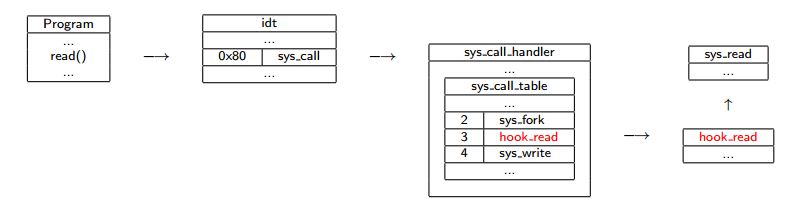
\includegraphics[width=\linewidth]{hook}
    \caption{System read() hooked}
    \label{fig:hookRead}
\end{figure}
basically, we call our function instead of the original read function. Within our function we call the original system read function, log the data we want and return the returned value of the the original system read.\
{\bf{Limitations: }} The read system call is widely used, it's not efficient to add a burden on the system with no need.
\subsubsection{Attaching to Keyboard notifiers (Our approach)}
{\bf{Idea: }}
The Linux kernel has a notification functionality provided through the file linux/notifier.h.
It's similar to the ``Observables" concept in web programming. 
The Kernel will trigger a call to a certain function when some action happens.
The keyboard driver uses this mechanism (notifier chains).
If a kernel subsystem wants to be notified on a certain action, it appends a notifier block to the list of blocks to be notified.
To add a function to the notifiers chain we have first to create a notify\_block as follows:\\\\
static struct notifier\_block nb = \{.notifier\_call = keyLogger\};\\
keyLogger is a pointer to the function that should be notified.

Now we can add our notifier block to the keyboard notifiers chain by calling:   \\register\_keyboard\_notifier(\&nb);\\

On each keystroke we will be notified with the keyboard\_notifier\_param that contains a value attribute that returns the key code of the key stroked and contains a down attribute that returns true if the key is pressed and false if the key is released.

Now we can determine which  key was pressed by creating an array to map keys to chars and handle Caps Lock and shift presses.

\subsection{Sending KeyLogs}
To send our keylogs, we first had to create a client socket using the kernel method sock\_create in sock.h 
We choos UDP to have less burden on the network and for it's simplicity  (KISS principle: Keep It Simple, Short).
For testing purposes, we choose to send our packets to the localhost (127.0.0.1)\\
Usually the systems assigns the socket a random source port for outgoing packets. Here we chose to bind it to make socket hiding a bit easier.

\subsection{Hiding Sockets}
After investigating the possible ways to list UDP sockets, we found that all socket and port capturing systems (ex: netstat) uses /proc/udp as their source of information. The proc filesystem contains sequence files (sequence files are files that get filled with information dynamically) with information about the sockets and ports used by the system. 
Now, our goal is to takeover the function responsible for showing the udp sequence files data .\\
In order to find that function, we had to iterate through the net namespace to find the proc\_dir\_entry for /proc/ProcessID/net (where ProcessID is the pid of the process using a socket).
After finding the proc\_dir\_entry for /proc/ProcessID/net, we can simply search for the udp file and get it's sequence file information (udp\_seq\_afinfo).
 using the udp\_seq\_afinfo we can reach the udp sequence show method (seq\_ops.show).
Finally, we can hook our function.\\
In our function we simply check the socket, if it uses a source or destination port that should be hidden we return 0 else we return what the original sequence file show method should have returned.
\clearpage
\section{Future Work}
\subsection{Dynamic socket hiding}
Instead of binding the source port of the keylogger udp packets, we can let the system assign a port dynamically and then we hide it.
\subsection{File Hiding}
By hooking the system call used by ls.
\subsection{Packet Hiding}
We would like to even hide the packets sent by the keylogger so that they are not visible in sniffing programs (ex: wireshark).
\subsection{Buffered KeyLogging}
Instead of sending each keystroke in a UDP packet, we could combine several keystrokes together, this would increase the bandwidth utilization and allow us to  capture and save offline keystrokes and send them when the user connects to the Internet.
\subsection{Magic Packet KeyLogging}
Instead of sending the packets right away, we can configure our system to send the keylogs only after receiving a certain packet (magic packet)
Also we can create magic packets to control what ports, files, processes,....etc. to be hidden or shown.
\subsection{Keylogging only useful information}
We can log only  useful keystrokes by inspecting the packets deeply and start keylogging only when we find that a secure connection is opened.
\clearpage
\section{References}
\begin{enumerate}
\item http://memset.wordpress.com/2010/12/28/syscall-hijacking-simple-rootkit-kernel-2-6-x/
\item http://althing.cs.dartmouth.edu/local/LKM\_HACKING.html\#I.1.
\item http://commons.oreilly.com/wiki/index.php/Network\_Security\_Tools/Modifying\_\\and\_Hacking\_Security\_Tools/Fun\_with\_Linux\_Kernel\_Modules\#Hiding\_Processes
\item https://github.com/psychomario/LinuxLKMRootkit/blob/master/lkm.c
\item https://github.com/mfontanini/Programs-Scripts/blob/master/rootkit/rootkit.c
\item https://github.com/joshimhoff/toykit/blob/master/toykit.c
\item http://www.gilgalab.com.br/hacking/programming/linux/2013/01/11/Hooking-Linux-3-syscalls/
\item http://www.catb.org/~esr/showkey/
\item http://info.fs.tum.de/images/2/21/2011-01-19-kernel-hacking.pdf
\item http://www.tdp.org/LDP/lkmpg/2.6/lkmpg.pdf
\item http://www.gadgetweb.de/programming/39-how-to-building-your-own-kernel-space-keylogger.html
\end{enumerate}
\end{document}

